\chapter{Theory of classification}
In this chapter some of the theory of classification is introduced. The discussion is constrained to binary classification, of which the Ford Challenge classifier, is an example. First a general problem definition is given and notation is introduced. Then two concrete examples of classification models are introduced (Logistic Regression and Neural Network), and similarities and differences between the methods are described. Finally a techniques to measure the performance of different classifiers are discussed, including AUC that was used as the grading method in The Ford Challenge.

\section[The binary classification problem]{The binary classification problem\protect\footnote{This section is loosely based on \citet[sec 22.1-22.2]{wasserman04}}}
In a binary classification problem a binary outcome $t$ must be predicted from a $d$-dimensional input vector $\ve{x}=[x_1, x_2, \dots, x_d]^T$. The input vector represents an event, and the outcome variable $t$ represents the assignment of the event to one of two classes.
\begin{Exa}
    In \TFC\ the input is an instant in a driving situation, and this input should be assigned to either the class alert, or the class not-alert. The input is represented by an 30-dimensional vector and the assignment to a class is represented by $t=0$ meaning not-alert and $t=1$ alert.
\end{Exa}
To make the prediction possible, a trainingset $\mathcal{T}$ is given consisting of $n$ pairs of input vectors and corresponding, known outcomes.
\[
    \mathcal{T} = \bigl\{\:(\ve{x}_i, t_i)\:\bigr\},\quad i=1\dots n
\]
Based on this trainingset, a classification rule $f$ is learned, that can predict the outcome, of yet unknown input vectors. Therefore a classification rule is a function $f\,:\,\R^d\to\{0,1\}$, that is used to make the prediction $t=f(\ve{x})$ on a new input. \par
A common way to obtain a classification rule is by the Bayes classification rule. First define $p_k(\ve{x})$ as
    \[
        p_k(\ve{x}) = P(t=k|\ve{x}),\quad k\in\{0,1\}
    \]
    and then the Bayes classification rule is defined by
    \begin{definition}\label{def:bayes-rule}
        The Bayes classification rule $f^*$ is given by
        \[
            f^*(\ve{x}) = \begin{cases}
                1 & \text{if}\quad p_1(\ve{x})>p_0(\ve{x}) \\
                0 & \text{else}
            \end{cases}
        \]
    \end{definition}
    Since $p_0(\ve{x})=1-p_1(\ve{x})$, the Bayes classification rule can also be written
    \[
        f^*(\ve{x}) = \begin{cases}
            1 & \text{if}\quad p_1(\ve{x}) > \frac{1}{2} \\
            0 & \text{else}
        \end{cases}
    \]
    By the Bayes classification rule we have got a theoretical classification rule. In practice the posterior class probabilities $p_0(\ve{x})$ and $p_1(\ve{x})$ are unknown, so the trainingset must be used to find some approximation for these probabilities.\footnote{Since $p_0(\ve{x})=1-p_1(\ve{x})$ only one of the probabilities actually needs to be estimated}  The problem of approximating a probability distribution from a given data set is a classic statistical problem. The next section gives one way to solve this problem.

\section{Parametric models and maximum likelihood}\label{sec:parametric-models-and-likelihood}
Two distinct ways to approximate the probability distribution $\Ptx$ is using either a parametric or a non-paramtric approach. The focus in this report is on the parametric approach. The distribution $\Ptx$, is therefore approximated by a distribution $\PtxHat$ restricted to a class of distributions
\[
    \mathcal{F} = \Bigl\{\,f(t|\ve{x},\ve{w})\,\Bigr\}
\]
where the distributions $f\in\mathcal{F}$ are uniquely identified by their parameter $\ve{w}=[w_1, w_2, \dots, w_k]^T$. By restricting the approximating distribution $\PtxHat$ to the set $\mathcal{F}$, the problem of approximating $\Ptx$ reduces to the problem of estimating the parameter $\ve{w}$.

\subsection{Maximum likelihood}
There exists some different techniques to estimate the parameter $\ve{w}$ in a parametric model.\footnote{See eg. \citet[Sec.9]{wasserman04}} In this section we look at the most common method for estimation of the parameter in a parametric model, namely the maximum likelihood method.\par
The approximation $\PtxHat$ of the posterior class probability is restricted to the class $\mathcal{F}$. Using a trainingset, the likelihood function is now defined as the probability of obtaining the data in the trainingset, given as a function of the parameter $\ve{w}$. More formally\footnote{Taken directly from \citet[p.122]{wasserman04}}:
\begin{definition}
    The likelihood function is defined by
    \[
    \mathcal{L}(\ve{w}) = \prod_{i=1}^n f(t_i|\ve{x}_i,\ve{w}),\quad (t_i,\ve{x}_i)\in\mathcal{T}
    \]
    and the log-likelihood function is defined by $\ell(\ve{w})$ = $\log\mathcal{L(\ve{w})}$.
\end{definition}
It is worth noticing that the definition of the likelihood function assumes that the $t_i$'s are independent random variables. An assumption that in the case of \TFC\ may be a bit questionable. This is due to the sequential nature of the Ford Challenge dataset, which makes it very likely that datapoints that are close to each other in time, are not independent.\par
Given the definition of the likelihood function, the maximum likelihood estimator is now defined by
\begin{definition}
    The maximum likelihood estimator $\mle$ is the value of $\ve{w}$ that maximizes $\mathcal{L}(\ve{w})$.
\end{definition}
Notice that as the logarithm is a monotonic increasing function, the maximum of $\mathcal{L}(\ve{w})$ is equal to the maximum of $\ell(\ve{w})$. This turns out to be handy, since the log-likelihood is often easier to work with than the likelihood function. \par
With these definitions it is now time to introduce two concrete examples of classification methods.



\section{Logistic Regression}
In the logistic regression the parametric form of the posterior class probability $P(t=0|\ve{x})$ is assumed to be
\begin{equation}\label{eq:log-def}
    P(t=0|\ve{x}) = \frac{1}{1+e^{-(\Lx)}}
\end{equation}
where $\ve{w}=[w_1, w_2, \dots, w_d]^T$. The function
\begin{equation}\label{eq:sigmoid}
    \sigma(a) = \frac{1}{1+e^{-a}}
\end{equation}
is called the sigmoid function and it will be used a number of times in the following sections. For later convenience it is noted that
\begin{equation}\label{eq:sigmoid-derivative}
    \frac{d\sigma}{da} = \sigma(1-\sigma)
\end{equation}
The fact that $P(t=0|\ve{x})$ is modelled by the sigmoid function, may seem a bit random, but comes from the fact that (with $p_0=P(t=0|\ve{x})$)
\begin{align*}
    p_0 &= \frac{1}{1+e^{-(\Lx)}} 
\end{align*}
can be written
\begin{align*}
    p_0 &= \frac{e^{\Lx}}{1+e^{\Lx}} \myimp \\
    p_0 + p_0e^{\Lx} &= e^{\Lx} \myimp \\
    \frac{p_0}{1-p_0} &= e^{\Lx} \myimp \\
    \log \frac{p_0}{1-p_0} &= \Lx
\end{align*}
And therefore the parametric form in \eqref{eq:log-def}, comes from the assumption that the log-odds of $p_0$ is linear in the input vector $\ve{x}$. \par
Now to find an expression for the likelihood function, the probability of getting the data in the trainingset must be expressed. For a given $\ve{x}$ the class will be class 0 with probability $P(t=0|\ve{x})$. If class 0 is defined as a ``success'' then $t$ given $\ve{x}$ is Bernoulli distributed with probability parameter $p=P(t=0|\ve{x})$. \par
With $p_i=P(t=0|\ve{x}_i)$ the likelihood function can be written as
\[
    \mathcal{L}(\ve{w}) = \prod_{i=1}^n p_i^{t_i}(1-p_i)^{1-t_i}
\]
where $p_i$ is implicit a function of $\ve{w}$. The log-likelihood function is therefore given by
\begin{equation}\label{eq:log-like-logistic}
    \ell(\ve{w}) = \sum_{i=1}^n t_i\log p_i + (1-t_i)\log(1-p_i)
\end{equation}
The maximum of the log-likelihood function gives the maximum likelihood estimator of $\ve{w}$, so the derivative of $\ell$ wrt. $\ve{w}$ needs to be derived. From equation \eqref{eq:sigmoid-derivative} it is seen that
\begin{equation}\label{eq:probability-derivative}
    \frac{\partial p_i(\ve{w})}{\partial \ve{w}} = p_i(1-p_i)\ve{x}_i
\end{equation}
and therefore
\begin{align*}
    \frac{\partial \ell(\ve{w})}{\partial\ve{w}} &= \sum_{i=1}^n t_i \frac{1}{p_i}p_i(1-p_i)\ve{x}_i + (1-t_i)\frac{1}{1-p_i}(-p_i)(1-p_i)\ve{x}_i \\
    &= \sum_{i=1}^n t_i(1-p_i)\ve{x}_i - (1-t_i)p_i\ve{x}_i \\
    &= \sum_{i=1}^n (t_i-p_i)\ve{x}_i
\end{align*}
To make sure it is a maximum the second derivative wrt. $\ve{w}$ must be found. Using \eqref{eq:probability-derivative}, the Hessian of the log-likelihood is found as
\begin{align*}
    \ve{H} = \frac{\partial^2\ell(\ve{w})}{\partial\ve{w}\partial\ve{w}^T} = - \sum_{i=1}^n p_i(1-p_i)\ve{x}_i\ve{x}_i^T
\end{align*}
which can be rewritten as an matrix equation, by introducing the matrices $\ve{X}$ and $\ve{P}$. $\ve{X}$ is an $n\times d$ matrix with the $i$'th row being $\ve{x}_i$ and $\ve{P}$ is an $n\times n$ diagonal matrix with $p_i(1-p_i)$ in the diagonal. The Hessian can then be written
\[
    \ve{H} = \ve{X}^T\ve{P}\ve{X}
\]
For any non-zero $d$-dimensional column vector $\ve{u}$, let $\ve{u}_x = \ve{X}\ve{u}$. Then $\ve{u}_x^T = \ve{u}^T\ve{X}^T$ and therefore
\begin{align*}
    \ve{u}^T\ve{H}\ve{u} = \ve{u}_x^T\ve{P}\ve{u}_x
\end{align*}
Since $0<p_i(1-p_i)<1$, $\ve{P}$ is a diagonal matrix with positive elements, so $\ve{u}_x^T\ve{P}\ve{u}_x=\ve{u}^T\ve{H}\ve{u}>0$ for any vector $\ve{u}$. Therefore the Hessian is positive definite and then $-\ve{H}$ is negative definite. From this it is seen that it is indeed a maximum that is found and that it is a concave optimization problem, so a single global maximum exists. \par
The maximum likelihood estimator can now be found by solving $\frac{\partial\ell(\ve{w})}{\partial\ve{w}}=0$, but since $p_i$ isn't linear in $\ve{w}$ the equation must be solved numerically. An effective algorithm called iterative reweighted least squares can solve this problem \citep[p.207]{bishop}.

\subsection{The decision boundary}
An important property of a classification method is how complex, the datasets the method can separate in the appropriate classes, can be. The decision boundary of a classification method gives some imformation about how well it separates input data. The decision boundary is the set of points in the input space that lays at the boundary between input points that are classified as class 0 and input points that classify as class 1.
\begin{Exa}
    A trainingset consists of $n$ $d$-dimensional input data $\ve{x}_i=[x_{1i}, x_{2i}, \dots, x_{di}]^T$ and corresponding classes $t_i$. Using logistic regression, approximations of the posterior class probabilities $\widehat{p}_k(\ve{x})=\widehat{P}(t=k|\ve{x}), k\in\{0,1\}$ are found. Using these with the Bayes classification rule gives
    \[
        f(\ve{x}) = \begin{cases}
            1 & \text{if}\quad \widehat{p}_1(\ve{x})>\widehat{p}_0(\ve{x}) \\
            0 & \text{else}
        \end{cases}
    \]
    The decision boundary is given by all $\ve{x}$ where $\widehat{p}_0(\ve{x})=\widehat{p}_1(\ve{x})$. But by the definition of the linear regression
    \[
        \log\frac{\widehat{p}_1(\ve{x})}{\widehat{p}_0(\ve{x})} = \Lx
    \]
    So for all points at the decision boundary the following holds
    \[
        \Lx = 0
    \]
    This shows that the decision boundary of the logistic regression is linear in the inputs.
\end{Exa}
The classification methods with linear decision boundaries, defines a family of classification methods with simple analytical and computational properties \citep[p.179]{bishop}. This simplicity comes at the cost of the models having a limited capability to separate complex data sets. 

\subsection{Model complexity}\label{sec:logistic-complexity}
Although the logistic regression has a limited complexity, its ability to separate complex datasets can be increased by introducing feature transformations. Instead of just fitting the logistic regression to the $d$-dimensional input $\ve{x}=[x_1, x_2, \dots, x_d]$, eg. the squared transformations of the elements $x_i$ can be added to the input. This gives the $2d$-dimensional input 
\[
    \ve{x}_e = [x_1, \dots, x_d, x_1^2, \dots, x_d^2]
\]
This gives nonlinear decision boundaries in the original input space, which increases the number of datasets that can be separated. Notice that the decision boundary is still linear in the extended $2d$-dimensional input space. Instead of introducing transformed, non-linear features in the logistic regression, other methods exists, that have the non-linearity build-in. One example of such a model is the Neural Network.


\section{The Neural Network}\label{sec:feed-forward-neural-network}
The Neural Network originated from an attempt to create a mathematical model of information processing in the human brain \citep[p.226]{bishop}. But the Neural Network turned out to be useful in many pratical applications, and it is now seen as a standard statistical model \citep[p.392]{hastie09}. \par
A neural network is made up of one or more layers and each layer consists of one or more perceptrons. The perceptron is the basic building block of a neural network and it is described next

\subsection{Perceptron}
A perceptron consists of one or more inputs represented by an input vector $\ve{x}$ with corresponding weights $\ve{w}$ and an activation function $f$. The activation function is assumed to be differentiable. The output from the perceptron is then
\[
    y = f(\ve{w}^T\ve{x} + w_0)
\]
The intercept value $w_0$ is added to make the model more flexible. It can be seen as the weight of an extra input that is always 1.
As a stand alone unit, the perceptron can implement linear classification methods, as eg. logistic regression. To emulate the behavior of a logistic regression, the activation function is chosen as the sigmoid from equation \eqref{eq:sigmoid}. The output of the perceptron is modelled as the posterior class probability $P(t=0|\ve{x})$, which gives
\[
    P(t=0|\ve{x}) = \frac{1}{1+e^{-(\ve{w}^T\ve{x}+w_0)}}
\]
Compared with the logistic regression model in equation \eqref{eq:log-def} it is seen that the two are identical. An error function can now be defined exactly as the log-likelihood in the logistic regression (see equation \eqref{eq:log-like-logistic}) and a maximizing weight vector can be found. \par
The perceptron by itself isn't much more complex than the logistic regression, and the decision boundary is still linear in the input space. The non-linearity is achieved when multiple perceptrons are combined in a network.

\subsection{Neural Network for binary classification}
\begin{figure}[ht]
    \centering
    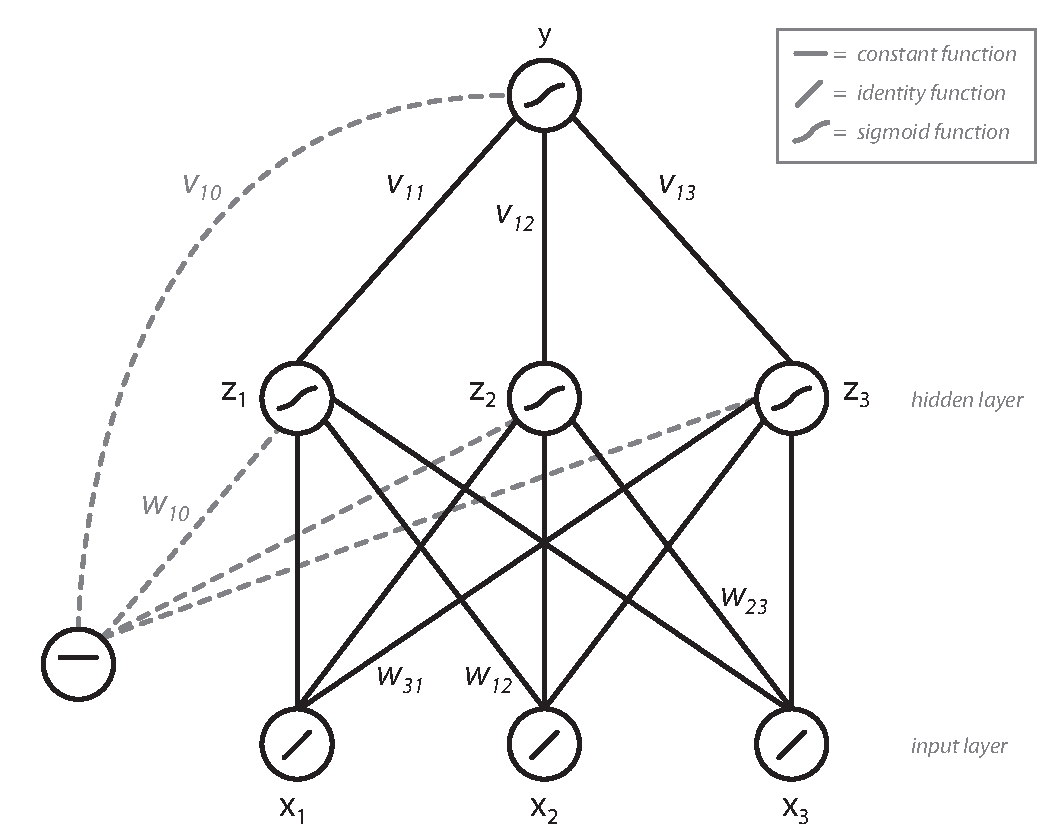
\includegraphics[width=110mm]{media/neural-network.pdf}
    \caption{Neural network}
    \label{fig:neural-network}
\end{figure}
In a neural network multiple perceptrons are combined, such that the output of one perceptron becomes the input of another perceptron. A lot of different network architectures exists but here the focus will be on feedforward networks with one hidden layer. \par
In a feedforward network the perceptrons can be divided into layers where the output of all perceptrons goes to a perceptron in the layer ``above''. The first layer is called the input layer and it consists of $D+1$ perceptrons, one for each feature in the input data, plus an intercept perceptron. The output of the input layer becomes input in the hidden layer, and each such connection has attached a weight $w_{hi}$. The hidden layer have $H+1$ perceptrons including an intercept perceptron. The output from the hidden layer, then becomes input to the output layer and each connection also has a weight $v_{1h}$. The output of the $i$'th perceptron in the input layer is $x_i$. The output of the $h$'th perceptron in the hidden layer is $z_h$ and is given by
\[
z_h = \sigma(\ve{w}_h^T\ve{x}+w_{h0}) = \frac{1}{1+e^{-(\ve{w}_h^T\ve{x}+w_{h0})}}
\]
assuming that the sigmoid function is used as activation function in the hidden layer. This is a common choice as activation function in the hidden layer, but other functions could have been used. The output of the hidden layer is sent to the output layer. Since the focus is on binary classification, the output layer consists of only one perceptron $y$. Since the output is modelled as the conditional probability $P(t=0|\ve{x})$, the sigmoid is also used as activation function for the output layer. The output can therefore be written
\[
    y = \sigma(\ve{v}_1^T\ve{z}+v_{10}) = \frac{1}{1+e^{-(\ve{v}_1^T\ve{z}+v_{10})}}
\]
From these expression it may be seen that the decision boundary is no longer linear in the output. To get a better sense for this, the output can also be written
\[
    y = \sigma\left(\sum_{h=1}^H v_{1h}\,\sigma\left(\sum_{i=1}^D w_{hi}x_i + w_{h0}\right)+v_{10}\right)
\]
The increased complexity of the neural network comes at a price though. Finding the weights that maximizes the log-likelihood is no longer a concave problem, in fact many maxima exists\footnote{See \citet[p.237]{bishop} for a description of how many, and \citet[p.297]{duda01} for a couple of graphs of the likelihood function}, and there are no guarantees that the global maximum will be found. Fortunately an efficient algorithm called backpropagation\footnote{See \citet[p.249]{alpaydin10} for an explanation of the backpropagation algorithm.} exists, that efficiently finds at least a local maximum.


\subsection{Model complexity}
In section~\ref{sec:logistic-complexity} it was described how the complexity of the logistic regression model, could be increased by adding transformed features. This can also be done in a neural network, but some other options exists as well. First of all different activation functions can be chosen for the different layers. In binary classification it is common to use the sigmoid function in the output layer, but the activation functions in the hidden layer can be freely chosen, and this may affect the complexity of the model. Another option is to increase the number of perceptrons in the hidden layer. As more perceptrons are added, the complexity rises with it. In fact it can be shown that any continous function can be approximated arbitrarily well by a network with one hidden layer, as long as enough perceptrons are added (see \citet[p.287]{duda01}).


\section{Measuring classifier performance}\label{sec:classifier-performance}
When a classifier has been trained on a training dataset, some estimate of the classifier performance, on future datasets, needs to be estimated. To be able to estimate the performance, it first needs to be defined exactly how the performance is measured. This can be done in many ways. For the Ford Challenge a measure called AUC-score was used.

\subsection[AUC]{AUC\protect\footnote{This section is loosely based on \citet[p.296-301]{kumar06}}}\label{sec:auc}
The AUC-score is the area under the Receiver Operating Characteristic (ROC) curve for a classifier, so to explain the AUC-score, an introduction of the ROC curve is needed. The ROC curve is based on four measures of the performance of a binary classifier. Assume that one of the two classes of the classifier have been labeled as ``positive''. Then the four measures are:
\begin{itemize}
    \item True positives (TP) - The number of positive samples that was correctly classified as positive.
    \item False negative (FN) - The number of positive samples that was incorrectly classified as negative.
    \item False positive (FP) - The number of negative samples that was incorrectly classified as positive.
    \item True negative (TN) - The number of negative samples that was correctly classified as negative.
\end{itemize}
From these four measures it is easy to calculate the true positive rate (TPR) and false positive rate (FPR) as
\[
\text{TPR} = \frac{\text{TP}}{\text{TP}+\text{FN}}\quad\quad\text{and}\quad\quad \text{FPR} = \frac{\text{FN}}{\text{TN}+\text{FP}}
\]
Based on the TPR and FPR measures an ROC curve can be calculated.

\subsubsection{Generating the ROC curve}
The ROC curve assumes that the classifier outputs continous-valued output and that the ordering of the output corresponds to the classifiers ranking of the inputs connection with the ``positive'' class. This is exactly the case when an estimate of the posterior class probability $P(t=0|\ve{x})$ is the output of a classifier. \par
To generate the ROC curve for a classifier on a specific trainingset, all rows in the trainingset are predicted by the classifier. Then the rows are ordered by these predictions. A threshold parameter is set equal to the highest prediction and all rows with a prediction lower than or equal to the threshold is predicted to belong to the negative class. For this threshold all rows are predicted as as negative, and therefore both TPR=0 and FPR=0 and therefore the point (0,0) is plotted on the ROC curve. The threshold is now set as the next lowest prediction and TPR and FPR are recalculated and the point (FPR, TPR) is plotted on the ROC curve. This is repeated until the threshold is equal to the lowest prediction, at which point all rows are classified as positive, and therefore the point (1,1) is plotted. The curve generated is the ROC curve which plots the relationship between FPR and TPR, as the threshold varies from lowest to highest prediction. \par
Two extreme examples will clarify what a ROC curve for a good classifier and a bad classifier looks like. If a classifier predicts all rows correctly it will rank all positive rows higher than the negative. As the threshold is lowered the TPR will rise to 1, while the FPR remains at 0. When TPR have reached 1, the FPR starts to go towards 1. The ROC curve for a perfect classifier therefore starts at (0,0), steeply rises to (0,1) and then goes to (1,1). \par
If the classifier on the other hand is just randomly making prediction the behaviour is different. When the ROC curve is generated the threshold at any time during the generation divides the dataset such that $p\cdot 100\%$ of the dataset is classified as positive. For a classifier that makes random prediction on a dataset with $n_+$ positive rows and $n_-$ negative rows, it would be expected that $pn_+$ rows will be classified positive and $pn_-$ as negative. This gives TPR$=(pn_+)/n_+=p$ and FPR$=(pn_-)/n_-=p$. So for all thresholds a point near $(p,p)$ is expected and as $p$ is updated every time the threshold is updated, the result is the straight line from $(0,0)$ to $(1,1)$. \par

\subsubsection{Good and bad AUC scores}
Based on the observations in the previous paragraph it is seen that good classifiers have an area under the ROC curve close to 1, while bad classifiers have areas around 0.5. This is used to measure the performance of different classifiers. When a classfier has been trained it makes prediction on a testset and the area under the ROC curve is calculated, and this is the AUC score of the classifier. \par
Some properties of the AUC score makes it appealing to use. It is a single number and no parameters are chosen by the person calculating the AUC, which means that different people, calculating the AUC of the same classifier on the same dataset should get the same value. Some problems with the AUC score exists though.
\begin{figure}[ht]
    \centering
    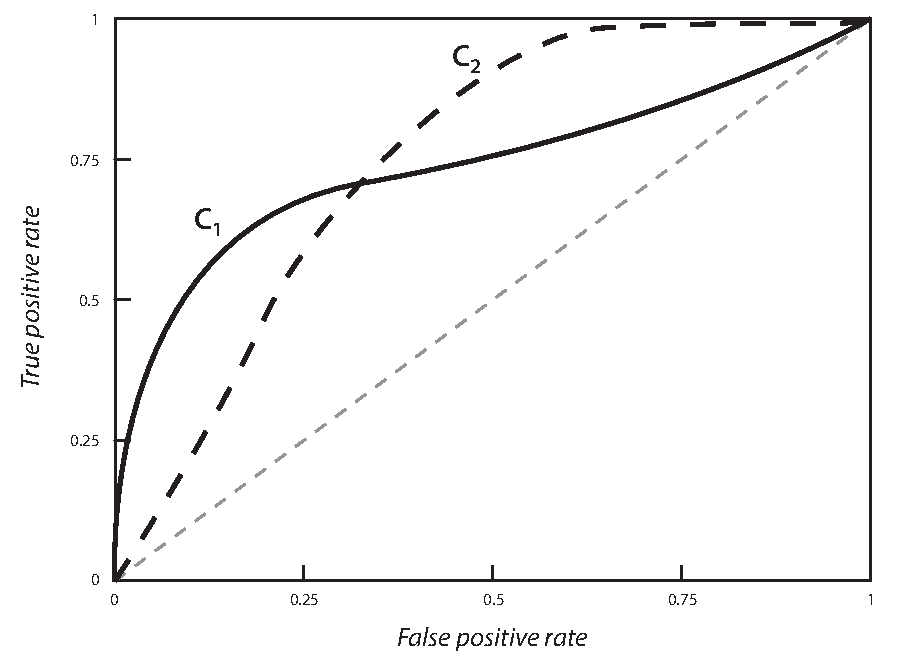
\includegraphics[width=110mm]{media/roc.pdf}
    \caption{Some examples of ROC curves. Although $C_2$ achieves a slightly higher AUC, $C_1$ may be prefered as discussed section~\ref{sec:auc-critique}}\label{fig:example-rocs}
\end{figure}

\subsection{Critiques of AUC}\label{sec:auc-critique}
The AUC for a classifier is calculated by letting the threshold value change from the lowest to the highest prediction. When a final model is chosen this threshold is set to a specific value, which means that the AUC score is influenced by behavior of the classifier that may never be of pratical interest. Take for example the ROC curves in figure~\ref{fig:example-rocs}. The classifier $C_2$ achieves the highest AUC, but $C_2$ performs worse than $C_1$ when FPR$<0.35$. In a pratical application a false positive rate above 0.35 may be totally unacceptable and then $C_1$ would be the prefered classifier. One obvious solution to this problem would be to only calculate the AUC for FPR$<0.35$, but this introduces a parameter that must be subjectively chosen, thus losing one of the advantages of the AUC. \par
A more profound critique of the AUC score shows that the relative cost of making a wrong positive prediction compared with the cost of a wrong negative prediction, depends on which classifier method the AUC is calculated for. See the paper \citet{hand09} for an indepth discussion. \par
The competition winner also mentions that the AUC score might be inapropriate for \TFC\ \citep[p.5]{inference_winning_approach}




\subsection{Cross validation}
When a measure has been chosen there still needs to be found a way to estimate the expected measure-score on future datasets, for the classifier. An emperical way to do this, is called cross validation. \par
One straight forward way to get an estimate of the expected performance on future datasets for a classification method, would be to measure the classifiers performance on the dataset used to train the classifier. The problem is that this will give an overly optimistic estimate, since the classifier has been trained to take into account some of the inevitable noise in the trainingset. To get a better estimate of the classifier performance, the complete dataset is split into smaller dataset, such that the same dataset is never used for both training and estimation of performance. This is the core idea in cross validation. Split the dataset to avoid using the same dataset for training and estimation. \par
The easiest way to split a dataset is to split it in two parts: a trainingset and a validationset. The classifier can then be trained on the traningset and its performance is estimated on the validationset. Although this technique works it use the dataset only once, and only one estimate of the performance is produced. This means that the variability in the estimate can't be estimated. If the validationset is large, it can be split in smaller subsets, and the performance can then be tested on each subset. This is the procedure used for this report, since the competition dataset had plenty of datarows. If only a small dataset exists a set of estimates can still be calculated by using $K$-fold cross validation. 

\subsubsection{$K$-fold cross validation}
In $K$-fold cross validation the dataset is split into $K$-parts. Then each part is selected as validationset once and the classifier is then trained on the $K-1$ remaining parts. This way $K$ values of the classifier performance is calculated, and these can be used to both estimate the expected classifier performance and the variablility in this estimate. It is worth noticing that this is not exactly the same as splitting a large validationset and calculating performance on each part. In that procedure only one model is trained on the validationset, while $K$ different models are trained in $K$-fold cross validation.

\subsection{Confidence interval of estimated performance}\label{sec:statistics-on-performance}
When $k$ measures of the performance of a model have been calculated, a confidence interval for the true value of the expected performance can be found. The $k$ measures are seen as a sample from the population of performance scores on future datasets, and this population is assumed normal distributed. For a small sample ($k<30$) with sample mean $m$ and sample standard deviation $s$, a $95\%$ confidence interval for the true mean $\mu$ can be found as\footnote{Section based on \citet[p.232-233]{johnson05}}
\[
    m-t_{0.025,k-1}\cdot\frac{s}{\sqrt{n}} < \mu < m+t_{0.025,k-1}\cdot\frac{s}{\sqrt{n}}
\]
where the value of $t_{0.025,k-1}$ can be found in a statistical table or in software as eg. \fn{R}. In this report the sample size will be $k=10$, which gives $t_{0.025,9}=2.2622$.

\section{Model selection}
As mentioned in the section about logistic regression and neural networks, the complexity of a model can be tweaked in different ways. A natural question is how complex the model should be chosen. Should the complexity be as high as is computational possible? Or should the complexity be kept as low as possible? As is often the case, the answer is that the complexity should be somewhere between low and high, which is explained by the concept of over- and underfitting. \par
If the model complexity is made as high as possible, the model will probably suffer from what is called overfitting. This means that the model has learned so many details from the training data, that it has adapted to the noise in the training data. Although this gives a great performance on the trainingset, it also means that the model will perform worse on future datasets. That is, the generalization of the model gets worse, when the fit to the trainingdata gets too high\footnote{See \citet[p.220]{hastie09} for a good illustration of overfitting.}. \par
At the opposite end of the scale is a model that is too simple. When a model is to simple it can't adapt to the patterns in the training dataset, that is shared with the future dataset. That way the model will neither fit the trainingset nor any future datasets. \par
One way to determine the right level of complexity is by using cross validation. By training models at different complexity levels and comparing their estimated performance, the right complexity can be chosen for the model.

\subsection{Forward feature selection}
One way to tweak model complexity, that is independent of the classification model used, is feature selection. In feature selection a subset of the whole set of features is selected for the classification model. Since the performance can depend on combinations of features, all possible subset of features should ideally be tested to find the optimal subset. For a high-dimensional input space this is not possible.
\begin{Exa}
    For the Ford Challenge the input data is 30-dimensional. This gives $2^{30}\approx10^9$ unique subsets to test. Since the model must be trained for each unique subset this is not a feasible solution.
\end{Exa}
Instead of trying every combination of features, different heuristics exists, that find a solution that is better than many alternatives. But optimality isn't guaranteed. One such heuristic is the forward feature selection. The procedure is simple. Start with a model that consists of no features and a set of candidate features that could be included in the model. Add the first candidate to the model and test performance. Then exchange the first candidate with the next and test performance, etc. The candidate that gives the best performance is removed from the candidate set and permanently added to the model. Recursively apply this procedure until the performance is no longer improved by adding features. \par
The forward feature selection is a greedy algorithm that at each stage selects the feature that gives the largest performance improvement. This doesn't guarantee an optimal performance but the worst case number of model training is (with $d$ features in the candidate set)
\[
    \sum_{i=1}^d i = \frac{d(d-1)}{2}
\]
The algorithmic complexity is therefore reduced from exponential $O(2^d)$ to polynomial $O(d^2)$.

